\pgfsetplotmarksize{0pt}
\begin{figure}
 \centering
 \caption{\label{fl_conv2}FLClustered/test2.txt},
 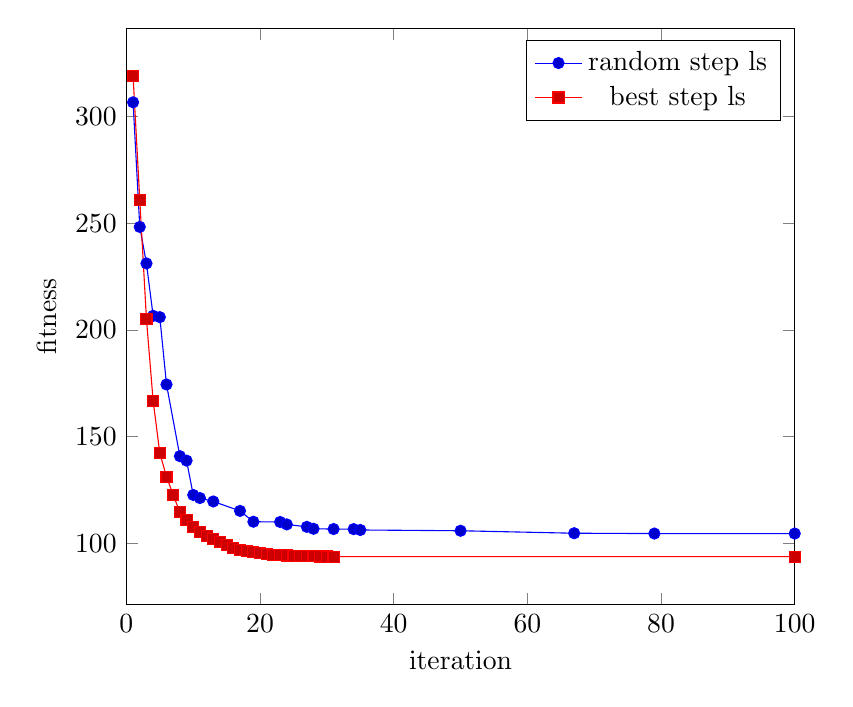
\begin{tikzpicture}
 \begin{axis}[
   width=0.7\textwidth,
   scale only axis,
   xlabel=iteration,
   ylabel=fitness,
   xmin=0,xmax=100,
   domain=0:100]
   \addplot coordinates {
     (0,inf)
     (1,306.762)
     (2,248.346)
     (3,231.256)
     (4,206.668)
     (5,206.049)
     (6,174.498)
     (8,140.892)
     (9,138.801)
     (10,122.702)
     (11,121.25)
     (13,119.654)
     (17,115.223)
     (19,110.15)
     (23,110.03)
     (24,108.899)
     (27,107.746)
     (28,106.84)
     (31,106.72)
     (34,106.686)
     (35,106.28)
     (50,105.918)
     (67,104.757)
     (79,104.607)
     (100,104.607)
   };
   \addlegendentry{random step ls}
   \addplot coordinates {
     (0,inf)
     (1,318.98)
     (2,261.014)
     (3,205.111)
     (4,166.817)
     (5,142.297)
     (6,131.291)
     (7,122.681)
     (8,114.664)
     (9,110.881)
     (10,107.81)
     (11,105.503)
     (12,103.542)
     (13,101.982)
     (14,100.477)
     (15,99.1097)
     (16,97.9013)
     (17,97.0523)
     (18,96.3395)
     (19,95.831)
     (20,95.3712)
     (21,94.9469)
     (22,94.6768)
     (23,94.4993)
     (24,94.3481)
     (25,94.2095)
     (26,94.0898)
     (27,93.9841)
     (28,93.9122)
     (29,93.8662)
     (30,93.8257)
     (31,93.7933)
     (100,93.7933)
   };
   \addlegendentry{best step ls}
 \end{axis}
 \end{tikzpicture}
\end{figure}
